\documentclass{article}
\usepackage[nonanonymous]{neurips_2026}

% Identify the course-project draft in the first-page notice.
\makeatletter
\renewcommand{\@noticestring}{CSCI 5150 Course Project. Draft.}
\makeatother

\usepackage[utf8]{inputenc}
\usepackage[T1]{fontenc}
\usepackage{hyperref}
\usepackage{url}
\usepackage{amsmath}
\usepackage{amsfonts}
\usepackage{graphicx}
\usepackage{microtype}
\usepackage{xcolor}
\setcitestyle{numbers,square,comma}

% Working title.
\title{Interpretable Risk Prediction\\for GPU Kernel Replacement}

\author{%
  WANG Zirui \\
  \texttt{ziruiwang@link.cuhk.edu.hk}
  \And
  ZHANG Juncheng \\
  \texttt{jczhang25@cse.cuhk.edu.hk}
}

\begin{document}

\maketitle

\section{Introduction}

Efficient GPU kernels are essential for delivering low-latency, high-throughput inference in modern large language model (LLM) serving systems.
The pursuit of higher kernel efficiency motivates replacing existing implementations with optimized alternatives.
However, optimizing kernels for GPU execution can change the order of parallel reductions, fuse multiply-add operations, or reduce the precision of intermediate accumulations.
These implementation choices alter how intermediate results are rounded and can produce numerical differences even when the computations are mathematically identical~\citep{whitehead2011precision,pytorchNumericalAccuracy}.
For LLM serving, the benefits of faster kernels also depend on whether model quality is preserved.

The impact of a numerical difference on model quality may depend on both the computation it changes and the task the model performs.
For example, a change in an intermediate representation is processed by subsequent layers, whereas a change in the final output scores occurs directly before answer selection.
We therefore investigate whether information about the task and the affected kernel's role helps predict changes in task outcomes beyond what discrepancy magnitude alone can explain.

To study this relationship, we estimate the probabilities of two outcomes: \emph{output change}, where the final task output differs from the reference execution, and \emph{negative flip}, where a prediction that was correct in the reference execution becomes incorrect.
We fit and select risk models using only data from controlled numerical perturbations of varying magnitudes, then test whether their predictions transfer to real kernel replacements.

Our interpretable risk model combines discrepancy magnitude with task, numerical precision, and kernel role.
Some combinations of these factors have few observations, making their risks difficult to estimate independently.
We therefore use partial pooling to share information across contexts while retaining differences supported by the data.

% Provisional closing sentence: replace the setting and verify this statement against completed experiments.
We implement and evaluate our approach on \texttt{[experimental setting]}, measuring prediction quality and coverage for real kernel replacements.

\section{Related Work}

\paragraph{Numerical stability in LLM inference.}
Prior work examines numerical error in low-precision attention~\citep{shah2024flashattention3} and the effects of execution configuration on LLM responses~\citep{yuan2025numerical}.
Kernel-level approaches improve reproducibility across batch sizes~\citep{he2025nondeterminism}, tensor-parallel configurations~\citep{zhang2026deterministic}, and GPU architectures~\citep{cooper2026mitigation} by controlling reduction order and arithmetic precision.
LLM-42 provides a decoding-level approach using verification and rollback~\citep{gond2026llm42}.
Our focus is on predicting the task-level consequences of numerical differences.

\paragraph{Prediction consistency and behavioral regression.}
Research on model update compatibility examines whether improved models preserve previously correct predictions, capturing regressions that aggregate accuracy can obscure~\citep{yan2021positive}.
Recent approaches reduce such negative flips through weight interpolation~\citep{schumann2024backward} and compatibility adapters for LLM updates~\citep{echterhoff2024muscle}.
Moving from mitigation to prediction, \citet{sheng2026regression} investigate inference-time signals for identifying regressions and find that their effectiveness varies across tasks and model updates.
Our setting keeps model parameters fixed and varies kernel implementations.

\paragraph{Risk estimation and calibration.}
Isotonic distributional regression provides a framework for probability estimation under monotonicity assumptions~\citep{henzi2021isotonic}.
Recent work on LLM calibration accounts for differences across prediction contexts: QA-calibration uses partial pooling across question--answer groups~\citep{manggala2025qa}, while multicalibration for code generation incorporates factors such as program complexity and language~\citep{campos2025multicalibration}.
\citet{wu2024bridging} further connect calibration across multiple groups to generalization under distribution shift.
Kernel replacement raises related challenges: data support varies across contexts, and the source of numerical error changes between training and evaluation.


\section{Methodology}
\label{sec:methodology}

Figure~\ref{fig:method-overview} summarizes the learning and evaluation workflow.

\begin{figure}[!htbp]
  \centering
  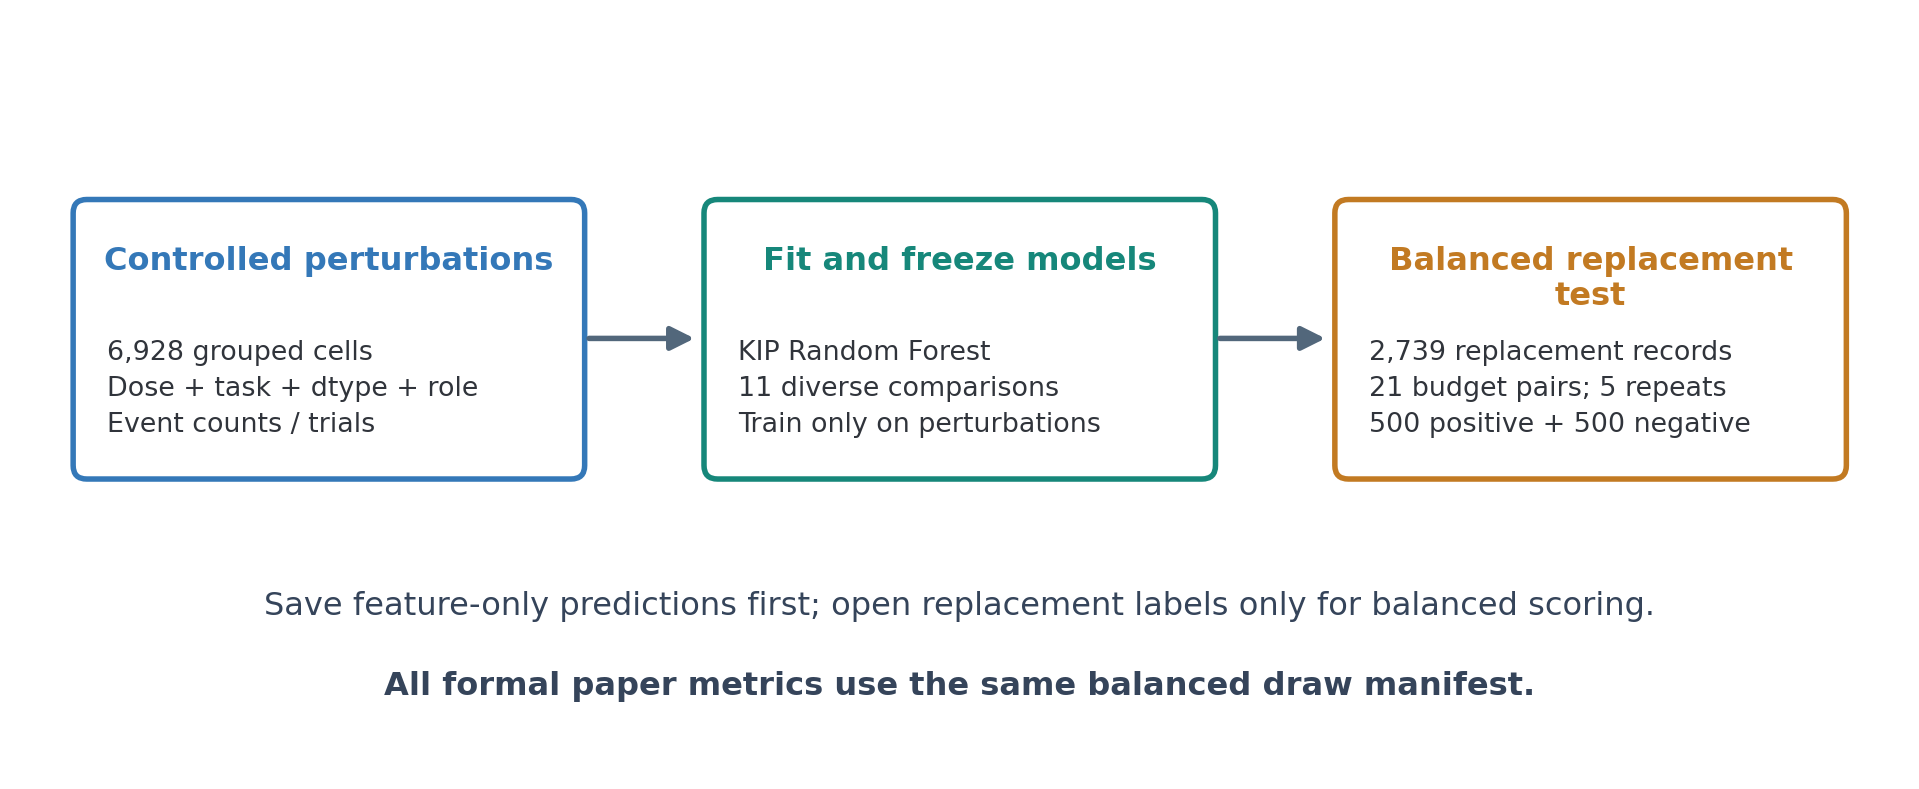
\includegraphics[width=\linewidth]{figures/method-overview.png}
  \caption{Risk estimation workflow:
  \textbf{(a)} fit and select models on controlled perturbations;
  \textbf{(b)} freeze the models and evaluate on real kernel replacements.
  All plots are schematic.}
  \label{fig:method-overview}
\end{figure}

\subsection{Problem Formulation}
\label{sec:problem-formulation}

We consider a model with fixed parameters.
For a task example $(x,y)$, let $f_{\mathrm{ref}}(x)$ denote the final output of the reference execution and $f_{\mathrm{alt}}(x)$ the output of an execution with a controlled numerical perturbation or a kernel replacement.
Let $C(o,y)\in\{0,1\}$ indicate whether output $o$ is correct according to the task's evaluation criterion.
We define two events:
\begin{equation}
\begin{aligned}
Z_{\mathrm{change}}
&= \mathbf{1}\!\left\{f_{\mathrm{alt}}(x)\neq f_{\mathrm{ref}}(x)\right\},\\
Z_{\mathrm{flip}}
&= \mathbf{1}\!\left\{
C(f_{\mathrm{ref}}(x),y)=1
\;\land\;
C(f_{\mathrm{alt}}(x),y)=0
\right\}.
\end{aligned}
\label{eq:risk-events}
\end{equation}
An output change occurs when the final task output differs from the reference output, while a negative flip occurs when a previously correct prediction becomes incorrect.

Let $d$ summarize the magnitude of the numerical change and let $c$ describe its computational context.
Our goal is to estimate
\begin{equation}
\begin{aligned}
p_{\mathrm{change}}(d,c) &= \Pr(Z_{\mathrm{change}}=1\mid d,c),\\
p_{\mathrm{flip}}(d,c) &= \Pr(Z_{\mathrm{flip}}=1\mid d,c).
\end{aligned}
\label{eq:risk-targets}
\end{equation}
These probabilities describe how often the corresponding events occur across task examples under the given numerical change and context.

\subsection{Data Representation and Features}
\label{sec:data-representation}

We summarize the controlled perturbation data as event counts for each experimental configuration.
A configuration is defined by the model, logical kernel, numerical precision, benchmark, and perturbation setting.
Each record $i$ contains the number of evaluated examples $n_i$ and the event count $k_{i,e}$ for each endpoint $e\in\{\mathrm{change},\mathrm{flip}\}$.
The corresponding empirical event rate is
\begin{equation}
r_{i,e}=\frac{k_{i,e}}{n_i}.
\label{eq:empirical-event-rate}
\end{equation}
Retaining both counts allows model fitting to account for differences in the number of examples supporting each observed rate.

For perturbation records, the magnitude $d_i$ is the upper bound of the applied perturbation range, represented as $\log_{10}d_i$ for positive values.
We encode task category, numerical precision, and kernel role as categorical features.
Kernel roles describe the function of the affected computation, such as normalization or output prediction.
We represent invocation count as $\log_{10}(1+v_i)$, where $v_i$ is the number of invocations per example, to distinguish computations that are affected once from those affected repeatedly during inference.

Model, candidate implementation, and benchmark identities are retained for data splitting and diagnostics but are excluded from the main predictor inputs.
In particular, the combination of model, logical kernel, precision, and benchmark defines an evaluation group, keeping records at different perturbation magnitudes within the same group.

\subsection{Context-Aware Risk Estimation}
\label{sec:risk-estimation}

For each endpoint, we fit a shared monotone risk curve and a regularized context adjustment.

\paragraph{Shared monotone curves.}
For each group $g$ defined by task category, precision, and kernel role, we estimate an event-probability curve over $z_i=\log_{10}d_i$.
Let $\mathcal{I}_g$ contain the records in group $g$, and let $\mathcal{M}$ be the set of nondecreasing functions taking values in $[0,1]$.
The shared curve for endpoint $e$ is obtained by weighted isotonic regression:
\begin{equation}
\widehat m_{g,e}
=\underset{m\in\mathcal{M}}{\arg\min}
\sum_{i\in\mathcal{I}_g}n_i\bigl[r_{i,e}-m(z_i)\bigr]^2.
\label{eq:shared-curve}
\end{equation}
We fit this curve using the pooled adjacent violators algorithm.
When a fine-grained group does not support a prediction, the hierarchy falls back to a task-level curve and then to a pooled curve.

\paragraph{Context adjustments and partial pooling.}
We learn context-specific adjustments from the features in Section~\ref{sec:data-representation}, shrinking estimates for sparse contexts toward their shared curves.
For output change, the design models whether any events occur and the event rate among records with at least one event.
Zero observed events are not equated with zero underlying probability.
For negative flip, the design uses a regularized grouped-binomial correction to the shared estimate.

\smallskip
{\small\noindent\textit{Draft note.}
The correction formulas, regularization penalties, fitting procedure, and fallback eligibility still need to be checked against the implementation.
The planned 13-role configuration also needs to be reconciled with the existing 17-role implementation.
Equation~\ref{eq:shared-curve} specifies monotonicity for the shared curves; monotonicity of the final corrected predictions has not yet been established.\par}

\subsection{Transfer to Real Kernel Replacements}
\label{sec:replacement-transfer}

For a real kernel replacement, let $\delta$ be the maximum absolute difference between reference and replacement kernel outputs evaluated on matched inputs.
We map $\delta$ to the tested positive perturbation upper bounds in $\mathcal{D}$.
For discrepancies within the supported range, we select
\begin{equation}
d^\star(\delta)=\min\{d\in\mathcal{D}:d\geq\delta\}.
\label{eq:dose-mapping}
\end{equation}
The fixed estimators take this mapped magnitude and the replacement's computational context as inputs.
This mapping does not by itself establish an upper bound on the true event probability.

The primary analysis includes replacements with a positive discrepancy, a supported magnitude, and the features required for prediction.
Let $\mathcal{R}$ be the set of unique replacement records and $\mathcal{S}\subseteq\mathcal{R}$ the subset satisfying these conditions.
We report applicability coverage as
\begin{equation}
\operatorname{Coverage}=\frac{|\mathcal{S}|}{|\mathcal{R}|}.
\label{eq:applicability-coverage}
\end{equation}
Zero-residual, below-range, above-range, and missing or unmatched records remain in the inventory and are reported separately.
They are not silently assigned a risk of zero.

\section{Experiments}
\label{sec:experiments}

% Leave empty until experiment artifacts and results are available.
% Add limitations after checking the implementation and empirical findings.

{
\small
\bibliographystyle{unsrtnat}
\bibliography{references}
}

\end{document}
